\documentclass[sigconf]{acmart}

\usepackage{hyperref}

%\usepackage{endfloat}
%\renewcommand{\efloatseparator}{\mbox{}} % no new page between figures

\usepackage{booktabs} % For formal tables

\settopmatter{printacmref=false} % Removes citation information below abstract
\renewcommand\footnotetextcopyrightpermission[1]{} % removes footnote with conference information in first column
\pagestyle{plain} % removes running headers


\begin{document}
\title{Unsupervised Learning For Detecting Fake Online Reviews}


\author{Syam Sundar Herle}
\affiliation{%
  \institution{Indiana University}
  \city{Bloomington} 
  \state{IN} 
  \postcode{47408}
  \country{USA}}
\email{syampara@iu.edu}
\bibliographystyle{ACM-Reference-Format}

\begin{abstract}
Nowadays decision making done by organization and individuals highly weighted on online reviews, social media opinions of any product or services. There is lot of valuable information available online, on which if proper mining technique is used we can reveal hidden values which are way useful to day to day life decision making. Given the usefulness of online data, individuals and group of people have started to take advantage of those data to boost up their business or products or creating an biased competition in market and this type of individuals and group of people create an opinion spamming system. Opinionated spamming are spams created by spammers to benefit their business fame or profit by giving biased reviews of product or service. Mechanism to detect these spammers or spam created by these spammers is an urgent need as we our technology has raised to new standard and raise in the rate of accessibility to online due to available technology. Here we are going to propose a such mechanism to detect fake review with help of an unsupervised machine learning model, which is trained using opinion mining of Natural Language Processing (NLP). Opinion mining is an art of extracting opinions of author, speaker or writer from their written text or spoken words, opinion mining is done by employing Natural Language Processing ,text analysis, Artificial Intelligence. 

\end{abstract}

\keywords{HID 219, Opinionated Spamming, Artificial Intelligence, Opinion Mining, Machine Learning, Natural Language Processing (NLP)}

\maketitle

\section{Introduction}

Usually the sentiment analysis can be defined as classifying a piece of written text into positive,negative or neutral state. This is also known as opinion analysis as it derives the opinion of the author. Said that, now a days, user's and consumers write reviews, opinions on online for a product or service given to them. The growth of web and internet has enabled user or consumers to communicate among each other and write up more reviews about products and has made the web more subjective and opinionated. As a result, huge amount of data in the form of texts are available from online which are rich in information, which are users review and opinion about products and service delivered to them. Which in turn can be used by the product owners to meet the consumer needs and demands, and provide quality products and identify the issues in products and much more. Unbiased and independent reviews about a product are the main decision making entity usually used by peoples while purchasing a product. 
Opinion mining is usually employed for the knowledge retrieval from textual contents such as review and comments. Opinion mining results the the textual content in one of the three categories namely positive, negative and neutral. Positive opinion are good in yielding good financial gains and fame and good business for product owners. On the other hand negative reviews helps in identifying the issues of the products, having said that some people usually write fake reviews to boost their financial gain or discredit their competitive product. These type of reviews are known as opinion spammers. In the following we will learn about sentiment analysis in detail and we will walk through some of the achievement done in detecting fake review and opinion spammers and we will propose our unsupervised learning model.
\section{Overview Of Big Data}
"Big Data describes a holistic information management strategy that includes and integrates many new types of data and data management alongside traditional data. 

While many of the techniques to process and analyze these data types have existed for some time, it has been the massive proliferation of data and the lower cost computing models that have encouraged broader adoption" \cite{bigdatadef}. Usually Big Data is comprised of four V's as said in \cite{bigdatadef} which is as follows,
\subsection{Volume}
Volume refers to the amount of data which are processed and stored, big data usually comprises of the high volume of low-level data which are granular in nature.

Real-time data captured from CCTV, internet live feed are so dense and has high volume, big data technologies allows user to convert these low-level high volume to high-level density data.
\subsection{Velocity}
The speed at which data captured can be defined here. As said in earlier sub-section data acquired from live feed CCTV are real-time in nature so the speed at which data are transmitted to the target storage also plays major role. Big Data requires processing and storage units to keep with the speed of the data being accumulated.
Traditional data storage cannot be used to handle Big Data. Big Data technology like Hadoop are required to store data.
\subsection{Variety}
The real nature or raw nature of the Big Data ranges from structured, semi-structured and unstructured. As the technology have grown, many unstructured data are being captured from social media, internet. Audio and Video files comprises to the most of the unstructured data. Big Data technologies are needed to convert these unstructured to structured data and process it. 
\subsection{Value}
According to \cite{bigdatadef} Data has intrinsic value, which are quantitative and textual in nature. Appropriate investigation method needed to derive the real value of the data to reveal the knowledge encapsulated in data which ranges from discovering a consumer preference or sentiment, to making a relevant offer by location, or for identifying a piece of equipment that is about to fail. The technological breakthrough is that the cost of data storage and compute has exponentially decreased, thus providing an abundance of data from which statistical sampling and other techniques become relevant, and meaning can be derived.

\section{Overview of Big Data Analytic}

Big Data analytic techniques are applied on large data to generate knowledge and reveal hidden patterns which can be harnessed to make useful in customer point of view. Now a days, Big Data analytic are used in many areas like DNA analysis, machine learning, deep learning, robotics and data classification.

The Big Data process can be broken down to two major component, Data Management and Data Analytic. In Data management segment the large set of data are acquired and recorder as first step, later the data are extracted from the storage or recorded devices and cleansed and annotated to meta file in the case of the unstructured data like video, text and audio. After cleaning and annotation the data are aggregated and presented in order to extract useful information. The unstructured data aggregated and integrated in this step to represent it as a structured data. In the next step Big Data Analytic are employed on the aggregated data, the first step of the analytic is the creation of model to apply on the aggregated data to perform analysis to reveal hidden value and pattern. In the next step visualization of the hidden pattern in the data is done and then the pattern are interpreted to make useful decision making to make a effective system for the consumer needs.

In the following subsection we will look into the available Big Data analytic for textual data.
 
 \subsection{Text Analytic}
 
 Extracting information from text data accumulated from social media, online questionnaire, survey and online feeds is known as Text Analytic. A number of analysis and model involved in text analytic like machine learning algorithm, natural language processing and linguistics. The following are the mining techniques are applied in the section of text analytic:
 
 
\subsubsection{Information Extraction}

These techniques extract structured meaning from the unstructured data. These techniques work in two sub task which are Entity Recognition(ER)\cite{bigdata} and Relation Extraction (RE)\cite{bigdata}.

\subsubsection{Text Summarizing}

As the name suggests these techniques create key points of single or multiple document in a succinct way. This analytic technique are employed in two ways, "Extractive Approach"\cite{bigdata} and "Abstractive approach"\cite{bigdata}. In the "Extractive Approach" summary is created from original statements and these summaries are subset of the original document by determining the salient points and putting them together. While the "Abstractive Approach" does the extraction of the semantic information from the text by employing Natural Language Processing techniques.

\subsubsection{Questionnaire}

These techniques provides answers to the questions, some of the edge of day applications are Apple Siri and Google Home\cite{bigdata}. Machine learning algorithm like deep learning and speech recognition and artificial intelligence are employed in the Questionnaire technique.

\subsubsection{Opinion Mining}

Opinion Mining are sentiment analysis, where Natural Language Processing and machine learning are employed to mine and classify emotion of the consumer in related to product or governance of a government. Usually text generated from online review portal or social media application like Twitter, Facebook are used to do sentiment analysis.


\section{Overview of Sentiment Analysis}

As defined earlier, sentiment analysis or opinion mining is the study of peoples opinion, attitude and emotion towards a product or any other entity. Usually the sentiment analysis is done on the textual contents like reviews of product, twitter tweets and comments in public blog about any entities. The overview of the sentiment analysis can be seen the Figure \ref{f:SA}.

\begin{figure}[!ht]
  \centering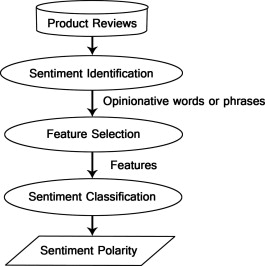
\includegraphics[width=\columnwidth]{images/sa.jpg}
  \caption{Sentiment Analysis on product review \cite{sentianalysis}}\label{f:SA}
\end{figure}

Overall, sentiment analysis is considered to be a classification process, which is done by three different types, the first one is being document sentiment analysis where the texts of documents are used to classify the opinion of the whole documents, the other type is sentence sentiment analysis where the texts of the sentence is used to classify the opinion of the sentence and third one is being aspect-level sentiment analysis where sentence or document are classified with respect to specific aspects of entity (product or service). 
\subsection{Data for sentiment Analysis}
In the first step of Sentiment Analysis, data are collected from online, the preferred data are reviews of product as these data are textual contents and unstructured and rich in information. These data are important in the sentiment analysis as the business owner can make use of the analysis of these data (review of product) to learn about users opinion about the product. The social media network are one of the good and important source of these types of data as users and consumers interact and post review of the products from their own accounts. 

The second important step is identifying the words or phrases which are useful in the forming the opinion in the sentence or document based on the type of sentiment analysis we intend to do as told in earlier paragraph. The following sub-section describes the next each steps in sentiment analysis in detail.

\subsection{Feature Selection}
The very important step in sentiment analysis is extracting features needed for the analysis, some of the feature selection used are,\textbf{Bag of Words and Frequency} in which a vector of binary is used as features, the binary vector comprises of 1 and 0 based on the presence of words in the document or sentence and forming a bag of binary vector for all words. The other weight used in these type of feature is the frequency of the words in the sentence or document. 

The next type of features used in sentiment analysis is \textbf{Part Of Speech} where the part of speech tagger is used to create features, in this method grammatical context tag of the words in sentence or document is used, these types features helps to find the emotion of the author from his or her texts.

The other features employed are \textbf{Opinion words and Negations} where features are built based upon the words which determines the words as bad or good and negation features gives overall appearance of the negative words in sentence or document.
\subsubsection{Feature Selection Methods} 
Here we can see some of the methods employed to extract and select features to perform sentiment analysis on the sentence or document. Usually feature selection can be done by two types of methods, \textbf{Lexicon-based} \cite{lexi} method and \textbf{Statistical-based} \cite{statis} method. The first method needs human annotation like bag of words (BOW) \cite{lexi} but the second method is usually is fully automated. Some of the statistical methods used in feature selection are given as follows,
\subsubsection*{Chi-Square $\tilde{\chi}^2$} : In chi-square test, the correlation between the term and categories is checked. According to \cite{sentianalysis} Consider n documents in any collection, and $p_{i}(w)$ be the conditional probability of class $i$ for document which contains the word $w$. and $P_{i}$ be the global fraction of document containing the class $i$, and $F(w)$ be the global fraction of document containing the word $w$. So the chi-square can be calculated as given in \cite{sentianalysis},
$$\tilde{\chi}^2 = \frac{n.F(w)^{2}.(p_{i}(w)-P_{i})^2}{F(w).(1-F(w)).P_{i}.(1-P_{i})}$$

The chi-square gives weights value for the words in the document and these value can be used as features for the sentiment analysis.

\subsubsection*{Information Gain} : In this method features are created based on the ranks of Information Gain entropy grouped in descending order. "The information gain usually measures the amount of information in bits about the class prediction, it also measures the expected reduction in entropy" \cite{Duch2006}.

\subsubsection*{Point-Wise Mutual Information} : This model provides mutual information between feature and classes, and this is derived from the information theory. According to \cite{sentianalysis} the point-wise mutual information, $M_i(w)$ is the information between the word $w$ and class $i$. So, we in laymen terms , the 
PMI \cite{sentianalysis} is the ratio between expected co-occurrence of class $i$ and $w$ which is given by $F(w).p_i(w)$ and the true occurrence which is given by $F(w).P_i$, so the PMI is defined as,
$$M_i(w) = log\bigg(\frac{F(w).P_i}{F(w).p_i(w)}\bigg)$$

The word $w$ is positive correlated to class $i$ if the value of $M_i(w)$ is greater than 0. Comparing with chi-square, PMI is not normalized value and hence for most of the feature selection chi-square is used.

\subsection{Classification Technique}

The classification technique employed for the sentiment analysis can be done by three approaches, Machine Learning approach, Lexicon based approach and use of both ML and Lexicon approach. In this sub-section we will walk through some of the techniques followed in all the three approaches.

\subsubsection{Machine Learning Approach}
Typical machine learning algorithms or predictive models are used in this approach, typically the ML approach can be divided into two models, Supervised learning and Unsupervised learning. 
\subsubsection*{Supervised Learning} : In supervised learning, a model is trained with the help of the labeled training data set and evaluated on the unseen data set which are known as test data set. After evaluating the test data classification accuracy are calculated to know how good the trained model is in classifying. Some of the supervised learning model used in sentiment analysis for classification techniques are,
\begin{itemize}
    \item Naive Bayes classifier : The Naive-Bayes is one of the probabilistic classifier, which works based on probabilities value to determine class. According to \cite{sentianalysis} the Naive-Bayes model predicts the posterior probability of a class to which the document belongs to, based on distribution of words in the document. For a given features it calculates the probability of the label assuming all the features $(f_i-f_n)$ are independent to each other, the Naive-Bayes follows the following equation to classify the class to which the document belongs to given the features, the features are generated by the Bag Of Words model.
    \begin{equation*}
        P(label/features) = \frac{P(label)*P(f_{1}/label)*.*P(f_{n}/label)}{P(features)}
    \end{equation*}
    As the above equation assumes the naive assumption of independence and uses Bayes theorem, it is known as the Naive-Bayes model.
    
    \item Support Vector Machine : Support Vector Machine model works based on the linear separation of the features which separates features in the search space to separate them based upon their classes, SVM is one of the linear classifier used in supervised learning ML approach. In SVM, the features are transformed to a higher dimensional state space and hyperplanes are used to separate the features, hyperplanes are determined by support vectors, which are features closer to the decision boundary of the separation of the features. For $n$ class of class the model needs $n-1$ support vectors. "SVM can construct a nonlinear decision surface in the original feature space by mapping the data instances non-linearly to an inner product space where the classes can be separated linearly with a hyperplane" \cite{sentianalysis}. In the case opinion mining, the classification are two positive and negative and hence one support vector is needed to do sentiment analysis.
    
    \item Neural Network : Neural Network (NN) consists of many basic unit which are known as neurons, the word frequencies in a document $X_i$ is given as input to the neuron, which has certain weights $A$ to compute probabilities values $P_i$ which is a product of $X_i*A$, the probability values acts as a linear function $f(.)$. So the linear function is given by,
    \begin{equation*}
    f(.) = X_i*A    
    \end{equation*}
    For the classification problem the linear function predicts the class label for the input $X_i$. The more the layer of neuron the better the output prediction will be, hence Multilayer Neural Network is employed in the classification problem if the number of class is more than 2.
\end{itemize}

\subsubsection*{Unsupervised Learning}
In the case of unsupervised learning, we will create a model to classify the classes of the data, the model is made to learn from the unlabelled data. In the case of sentiment analysis, analysis is done based on the similarity of the text and clustering them. Some of the unsupervised learning approach used in sentiment analysis are, 
\begin{itemize}
    \item LDA :  Latent Dirichlet allocation model is generative statistic model, Xianghua and Guo \cite{XIANGHUA2013186} used LDA model to automatically discover the aspects discussed in Chinese social reviews and also the sentiments expressed in different aspects.
    \item k-means : k-means employ metric to calculate distance between features created by bag of words (BOW) to cluster the words. 
    \item Cosine Similarity: Based on cosine similarity of word vectors, the textual content are grouped. In the case of any detection mechanism the target variables are detected by visualizing the pattern formed by the target variables.

\end{itemize}

\section{Related Work}

In this section we are going to walk through some of related work in detecting fake reviews, in \cite{7873647} an unexpected review pattern was studied and in \cite{6137345} an graph based model was studied to investigate the fake review detection. An supervised learning model was introduced in \cite{8026958} to study the detection of individual fake reviewers, by using duplicate reviews and near duplicate reviews as ground truth of fake review to classify the unseen reviews. As the labeled set was duplicate, the learning model was not able to give good accuracy of predicting the fake reviewers. In \cite{7873647} product review data was used to build a supervised learning model, the features for the model was based on the review text and product information to distinguish between duplicate review and non duplicate reviews. In \cite{7726174} fake review detection was done using the semantic and emotional model. In \cite{7822945} a semi-structured learning model was used to detect online deceptive detection, for this they used sentiment polarity and part of speech of words with linguistic inquiry word count  to create a supervised model to learn to classify the fake reviews and used the same features given to the model to create an unsupervised model to classify fake reviews.

In \cite{8026965} a semi supervised learning model was created in two phases, where in first phase a Naive Bayes classifier was trained with the labeled data set and in the semi supervised phase they incorporated they created an unsupervised learning model with the features of Naive Bayes and used EM algorithm to create a SGD to classify the fake reviews.  In this work they used product review data from Amazon product review and used FIM \cite{8026965} to train the Naive Bayes in the phase 1 and used precision, recall and F1-score as performance metric to evaluate SGD.

For sentiment analysis, sentiment lexicon or opinion lexicon is needed to classify the text into the different groups which is positive,negative and neutral. One of the method using the opinion lexicon to do sentiment analysis on the text is meta-level feature \cite{BRAVOMARQUEZ201486}. In this method, sum on the positive word and sum on the negative word are calculated to classify the text into specific opinion. As this method is manual in nature, a method based on genetic algorithm is proposed in \cite{KESHAVARZ20171} ALGA : Adaptive Lexicon learning using Genetic Algorithm, which creates opinion lexicon dynamically and addresses the manual problem and optimization problems in meta-level feature. But in case if big data is used in sentiment analysis then, ALGA results will be bad, in order to address this, big data analytic technology need to be incorporated \cite{bigdatainsenti}. According to \cite{bigdatainsenti} the runtime problem in \cite{KESHAVARZ20171} is tackled by using MapReduce framework of Big Data, by dividing the jobs of calculating scores of positive lexical and negative lexical into independent tasks and run them in parallel on large-scale cluster. In MapReduce framework program, the input data are partitioned into independent set and in Map program the independent set are compiled to produce key and value tuples where key is the word and value is the frequency of the respective word and in the Reduce program the tuples are combined. By doing so, the computational time ALGA \cite{KESHAVARZ20171} is reduced. 

Using bigger data usually requires more memory and also more computation time. In order to address this issue, Apache Hadoop \cite{hadoopsenti} was used to store data in efficient manner. Hadoop consists of HDFS file system and MapReduce engine that manages the data storage blocks. HDFS consists of Namenode and Datanode \cite{hadoopsenti} where the Namenode manages all the Datanode and as said earlier MapReduce deals the parallel processing of the data with the help of the master node and slave node. For various classification and clustering problem on the huge data, Apache Mahout \cite{hadoopsenti} is used. For the evaluation process in \cite{hadoopsenti} Apache Mahout splits the data set into training set and test set. The training set is used to train the classifier.

For spotting fake reviews via collective positive-unlabeled learning \cite{7023420} they used a Iterative Classification Algorithm ICA \cite{7023420} on reviews data to create features for the Multi-typed Heterogeneous Collective classification algorithm for the classification problem. As this was an classification problem they used labeled and unlabeled data set.

\section{Proposed Work}
The main goal of our proposed work is to detect opinion spammers, if we are going to employ a supervised learning as discussed in related work section we will be needing a labeled data set. But most of the data sources available on online are unstructured data without any labels for the fake reviews, in \cite{8026958} they used duplicate review as ground truth for classifying the fake reviews but the accuracy of proposed system in \cite{8026958} will be very low. If we want to create a labeled data set then we have to create a labeled data set Amazon Mechanical Trunk \cite{6681365} or segregate opinion groups manually. Even though both the process of creating labeled data set are easy to implement, they have their own disadvantages. Both mentioned process are expensive and industrious to implement. 

As there is a scarcity of labeled data set available for reviews, we will create an unsupervised learning as proposed in \cite{originalPaper} to detect fake review on the non-labeled data set using cosine similarity approach. In this section we will explain more about the data and feature generation technique which was employed and about main algorithm.

\subsection{Data}
For the proposed work we have used data from the Yelp Dataset Challenge which includes data from the Phoenix, Las Vegas, Madison, Waterloo and Edinburgh, with 42,153 businesses and 1,125,458 reviews. Yelp uses its own filtering algorithm to remove fake data set, but we will try to examine the effectiveness of their algorithm by our proposed novel method. The data is rich information and we have handle the data to process the data. The Yelp Dataset Challenge comprises of lot of data but we will be using two json files of the data, 'business.json' and 'review.json'.  From \cite{yelpdatasetchalleng} we can see the description of the data set, the 'business.json' file has all the information about the hotel like name, business id, address and so more. Whereas the file 'user.json' has all the information about the user like review,user id, business id, stars, rating and lot more.
\begin{figure}
  \centering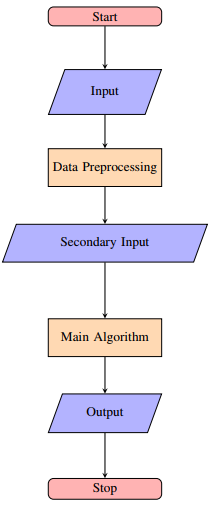
\includegraphics[scale=1.0]{images/Capture.png}
  \caption{System Architecture \cite{originalPaper}}\label{f:archi}
\end{figure}

From the architecture detailed in \ref{f:archi}, we can see that the input data is formatted to create a feature data set which can be used by the main algorithm later on.

\subsection{Feature Selection}

For the feature selection of our work we will employ cosine similarity method using Spark in python 2.7 and we will extract features needed for the model from the data set. As in \cite{originalPaper} we will create a dictionary for business id are created along with the business name from the 'business.json' file by iterating through all the rows of 'business.json' file. There may be some duplicates among the business id, so creating a dictionary will eliminate the probability of including the same encrypted business id again and again.

In the next step as in \cite{originalPaper} we have to iterate through all the rows of the 'user.json' file to grab the user review and rating along with the encrypted business id to which the user have given the rating and review. The very next step will be mapping the review and rating for the encrypted business id by looking up the encrypted business id of the dictionary file created in step one. We will create a folder named as business name and we store the reviews for the business name as individual text files and we will create a file with the name of business name having all the reviews for that business.

After completing this steps we will try to dump all the review files and rating files in rating and review main folders.

Now we have to form a word vector for each read file from review folder, iterate through business folder and read two text files and create two word vector for both files, after creating word vector along with the frequency for the words which are unique on both text files.  

\subsection{Idea behind Algorithm}

The main algorithm or unsupervised learning model which we are going to use in our work is proposed in \cite{originalPaper}, a cosine similarity. Assume if we have a data of a hotel delivering continental food and if a reviewer is writing 'The wine brewed and delivered in this place is so good', this gives us a suspicious as the place which is good for continental food but a reviewer has written about brewing and delivering of wine in a positive polarity. If this reviews cosine similarity is calculated with respect to other it will come in the range of 0.028 where other reviews will be in the range from 0.1 to 1. And the low cosine value is reinforcing our assumption that low cosine value will make it fall into category of opinionated spam or fake review.

\subsection{Unsupervised Learning Model}

The main unsupervised learning model or unsupervised algorithm we will be using is cosine similarity of reviews among them. As in \cite{originalPaper} the word vector of review file is taken as input to calculate the cosine similarity. Let us first give basic notation and mathematical expression involved in developing our unsupervised learning model.

\begin{itemize}
    \item Let \(r_1,r_2,.,r_n\) be n rating of user n for a specific business with the maximum rating of 5.
    \item Let \(N\) be the total number of users.
    \item Let the cosine similarity of the reviews of user n among other user reviews be \(c_1,c_2,..,c_n\).
\end{itemize}

The mathematical function for calculating the rating similarity as given in \cite{originalPaper},
\begin{equation}
    r_{Sim_{n}} = \frac{\sum_{i=0,k=0,i!=k}^{N}(r_i*r_k)/5}{N} \in [0,1]
\end{equation}

The mathematical for calculating the average cosine similarity is given by as follows,
\begin{equation}
    c_{Sim_n} = \frac{\sum_{i=0,k=0,i!=k}^{N}(c_i*c_k)}{\sqrt{\sum_{i=0}^{N}c_i^2}* \sum_{k=0}^{N}c_k^2} \in [0,1]
\end{equation}

The average cosine similarity gives the average cosine value of all reviews with respect to other reviews in specific business. The cosine similarity will be in the range of 0 to 1 and cosine similarity which are low are considered to be fake or opinionated spam for that specific business. The rating similarity is calculated because this gives us the expression of the reviewer for that specific business and we can find the specific review and rating is opinionated based on the average value of cosine and the rating similarity score.

\subsection{Results}

From the calculated average cosine and rating similarity values we can plot a 2-D plot to showcase our results as shown in \ref{f:op}

\begin{figure}[!ht]
  \centering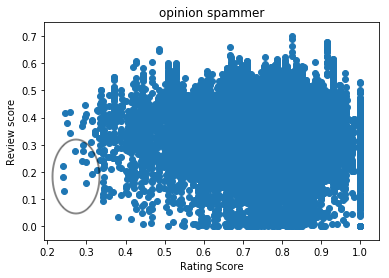
\includegraphics[width=\columnwidth]{images/sample.png}
  \caption{Result \cite{originalPaper}.}\label{f:op}
\end{figure}
From the 2-D plot \ref{f:op} we can see highlighted black oval shape on the scatter points which have low cosine similarity values and those are the fake reviews. From our noble unsupervised learning we were able to detect 10 fake reviews out of 1000 reviews from the filtered yelp data set.

\subsection{Information about machine environment}
The unsupervised learning model was executed on the local machine Virtual-Machine of Ubuntu 16.04 operating system having 2 GB RAM and Intel i7 processor. The model was also executed on Chameleon cloud of Ubuntu 16.04 and 2 gb ram, using one node.

\begin{figure}[!ht]
  \centering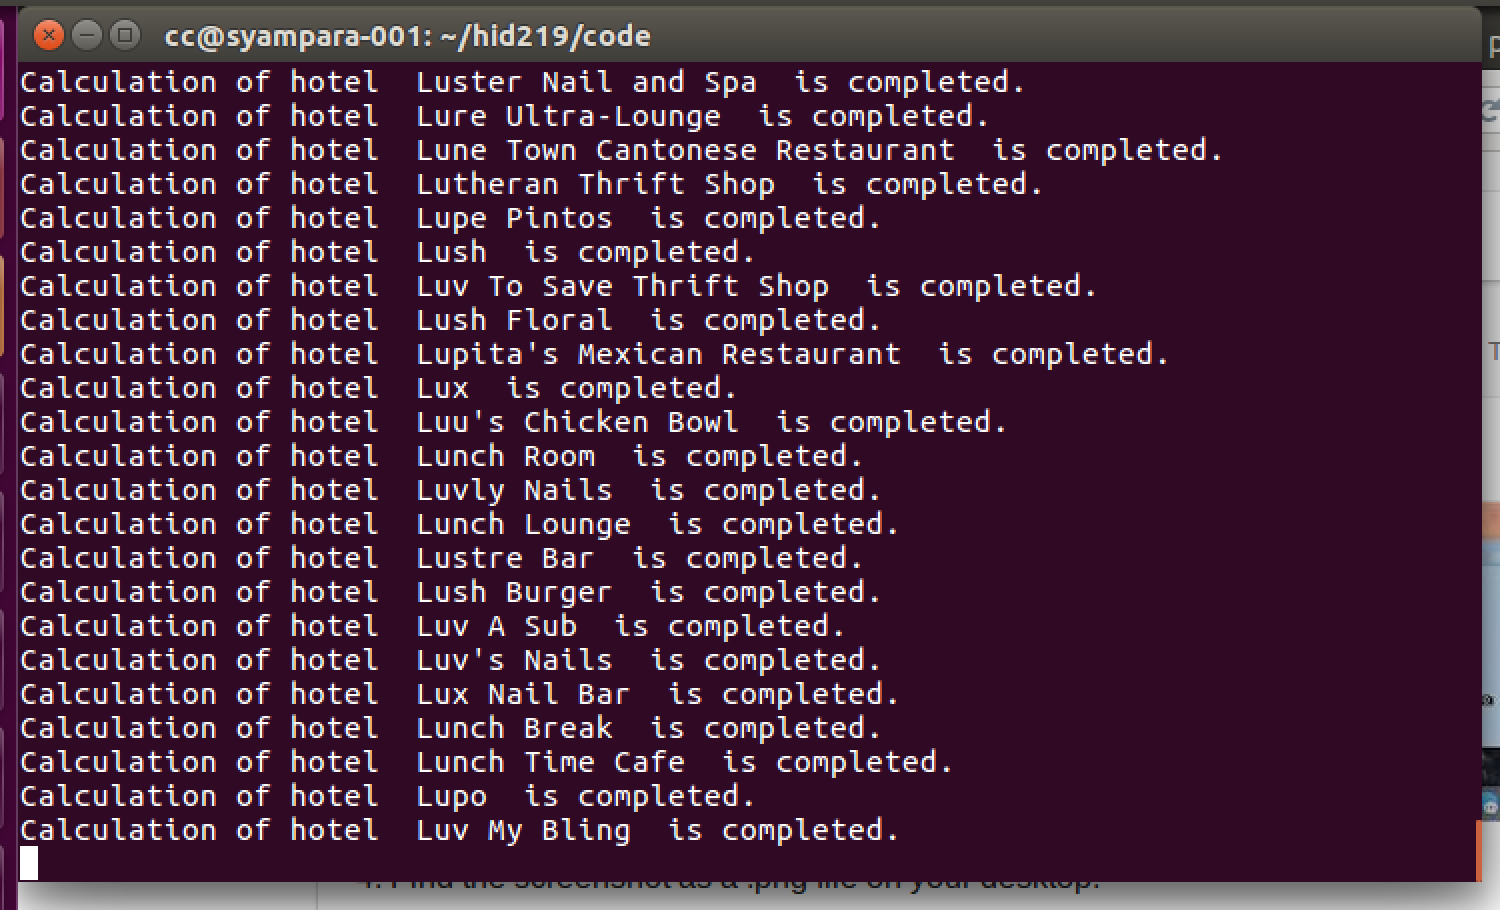
\includegraphics[width=\columnwidth]{images/chamcloud.png}
  \caption{Execution of model on Chameleon Cloud}\label{f:chameleon}
\end{figure}

From the figure \ref{f:chameleon} we can see the execution of the unsupervised learning model on chameleon.

Furthermore the model was also executed on bigred2.
\section{CONCLUSION}

We came across about Big Data and Big Data analytic in detail and we also came across about sentiment analysis in detail. Further we saw some of the related works of fake review detection using supervised learning, semi-supervised learning and unsupervised learning. We did an unsupervised learning model which works on cosine similarity as proposed in \cite{originalPaper} and we were able to detect some of the fake reviews like 10 out of 1000 in the filtered Yelp Dataset Challenge. 



\bibliography{report}  


\end{document}
